\setbackground
{
	\centering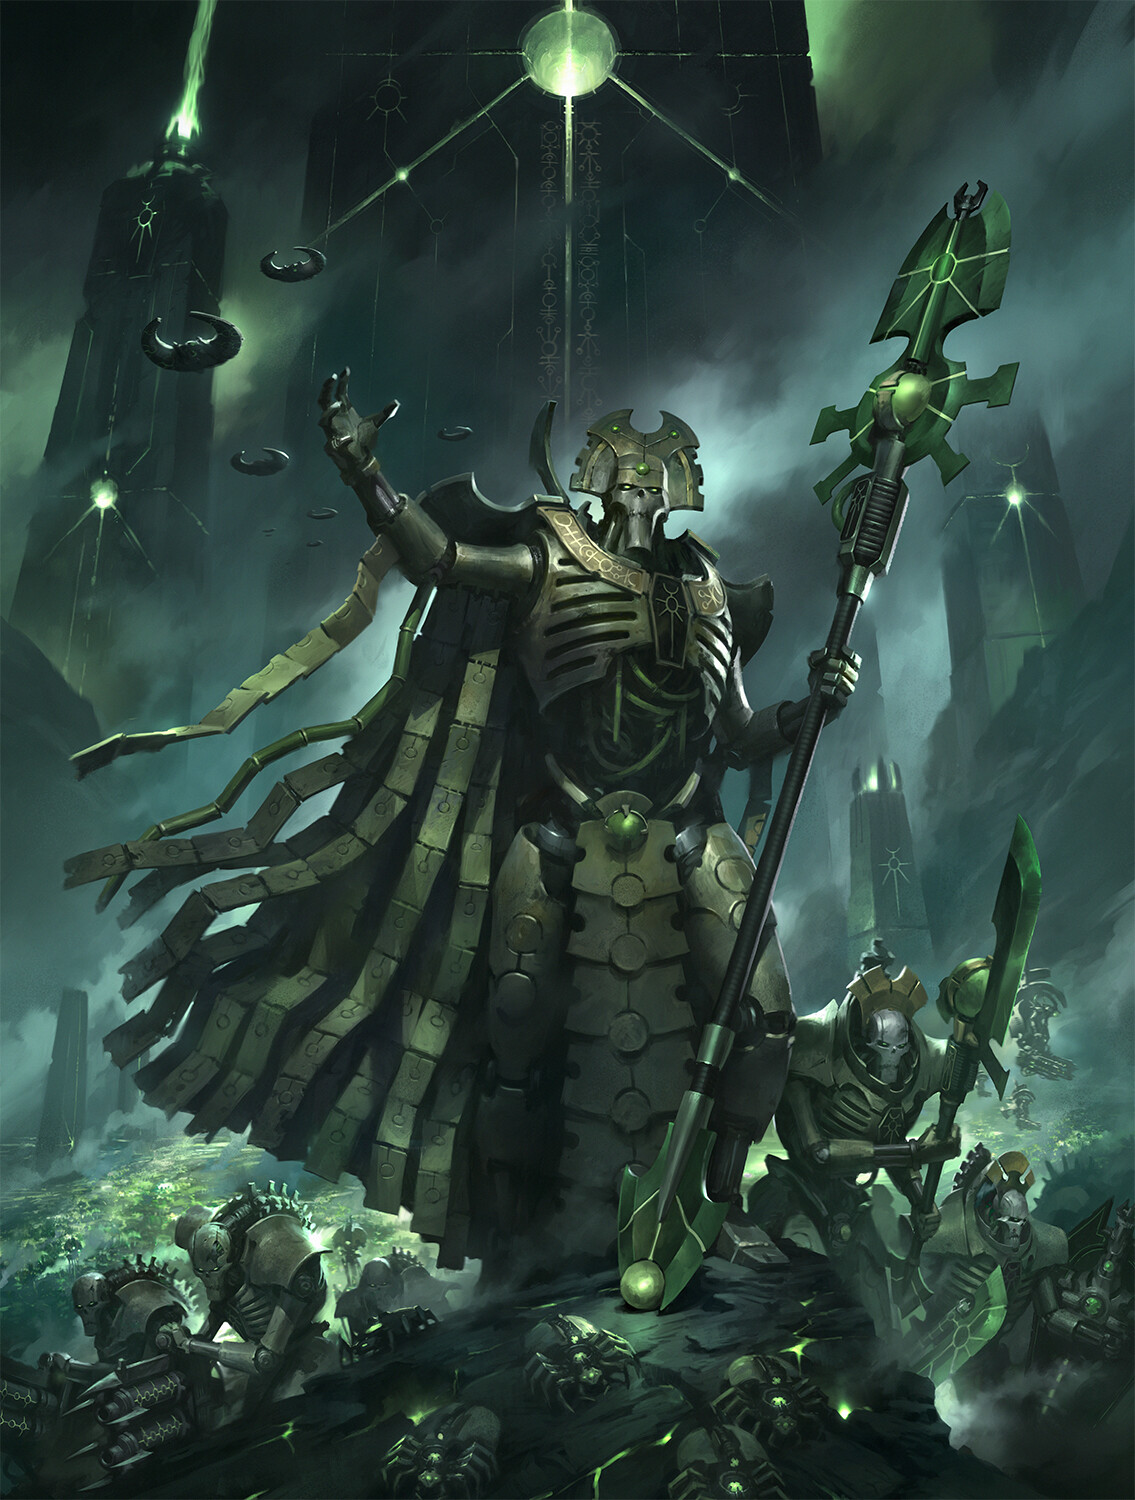
\includegraphics[height=530pt, width=400pt]{hq_art.jpg}
	\subsection[HQ]{\texorpdfstring{\centering\Huge HQ}{HQ}}
	
	\centerline{\begin{minipage}{400pt}
			\centering
			'You stupid bastard, you got us box seats to a coup.’
			
			‘Well, the reviews were very good.'
			
			\vspace*{1em}
			\raggedleft Orikan the Diviner to Trazyn the Infinite
	\end{minipage}}
}

\newpage
\clearbackground

\subsubsection[Lord]{}

\fbox{\begin{imgminipage}{marble.jpg}[t][0.90\textheight]{0.2\textwidth}
		\color{white}
		\centering {\large HQ}
		
		\raggedright \small
		A Necron Lord serves as the
		commander and primary Nodal
		point for much larger Necron
		armies. When the Necrontyr gave
		up their organic bodies, they
		transferred their consciousnesses
		into bodies made of the living
		metal Necrodermis. However,
		they soon discovered that over an
		extended period of time, their
		new robotic bodies dulled their
		minds and their ability to feel any
		type of emotion or pleasure.
		Over many millennia, the
		ultimate outcome of this process
		of gradual desensitisation was
		that the Necrons became soulless
		warrior-slaves.
		
		Only the most powerful and
		strong-willed of the nobility
		managed to gain access to
		Necrodermis bodies following
		biotransference that were
		sophisticated enough to allow
		them to maintain their full
		sentience. All are high-ranking
		members of a Necron dynasty's
		noble hierarchy and are usually
		placed by the dynasty's Phaeron
		or their own Overlord in control
		of an entire Tomb World. Clad
		in crumbling vestments and
		wielding ancient, arcane staff
		weapon, the Necron Lord is a
		chilling sight to behold on the
		battlefield as they direct their
		Warriors in unnatural silence.
		Their ancient metallic bodies are
		marred by the patina of age and
		they wear the accumulated power
		of millennia like a robe.
		\color{black}
\end{imgminipage}}
\hspace{0.5em}
\begin{minipage}[t]{0.72\textwidth}
	{\large \textbf{Lord \dotfill 75 Points}}
	
	\begin{tabular}{m{160 pt} *{10}{c}}
		& M & WS & BS & S & T & W & I & A & Ld & Sv \\
		\hline
		Lord & 7 & 4 & 4 & 5 & 5 & 2 & 2 & 2 & 10 & 3+ \\
	\end{tabular}
	\small
	\begin{minipage}[t]{0.5\textwidth}
		\begin{flushleft}
		\vspace*{2em}
		\textbf{Unit Composition}
		\begin{itemize}
			\item 1 Lord
		\end{itemize}
		
		\textbf{Wargear}
		\begin{itemize}
			\item \quickref{Staff of Light}
		\end{itemize}
		\end{flushleft}
	\end{minipage}
	\begin{minipage}[t]{0.5\textwidth}
		\begin{flushleft}
		\vspace*{2em}
		\textbf{Unit Type}
		\begin{itemize}
			\item Infantry (Character, \quickref{Living Metal}, \quickref{Noble})
		\end{itemize}
		
		\textbf{Special Rules}
		\begin{itemize}
			\item \quickref{Command Protocols}
			\item \quickref{Nodal Command} (Bronze)
			\item \quickref{Reanimation Protocols}
			\item Relentless
		\end{itemize}
		\end{flushleft}
	\end{minipage}
	
	\vspace*{2em}
	\textbf{Weapons}
	
	\begin{tabular}{m{90 pt} c C{40pt} *{2}{c} >{\raggedright\arraybackslash}p{130pt}}
		& Range & Type & S & AP & Abilities \\
		\hline
		\quickref{Staff of Light} & & &  &  &  \\
		— Shooting & 18" & Assault 3 & 5 & 3 & — \\
		— Melee & — & Melee & User & 3 & Rending (6+) \\
		\quickref{Hyperphase Sword} & — & Melee & User & 3 & Rending (5+) \\
		\quickref{Voidblade} & — & Melee & User & 4 & \quickref{Entropic Strike} (4+), Rending(6+) \\
		\quickref{Warscythe} & — & Melee & +2 & 2 & Armourbane (Melee), Two-Handed \\
		\quickref{Relic Gauss Blaster} & 30" & Rapid Fire & 5 & 4 & \quickref{Gauss} (6+), Twin-Linked \\	
	\end{tabular}
	
	\vspace*{2em}
	\textbf{Options}
	\begin{itemize}
		\item The Lord may exchange their \quickref{Staff of Light} for one of the following options:
		\begin{itemize}			
			\item \quickref{Hyperphase Sword} \dotfill -2 points
			\item \quickref{Voidblade} \dotfill +0 points
			\item \quickref{Warscythe} \dotfill +20 points
			\item \quickref{Warscythe} with in-built \quickref{Relic Gauss Blaster} \dotfill +30 points
		\end{itemize}
		\item The Lord may take any of the following options:
		\begin{itemize}
			\item \quickref{Aeonic Beacon} \dotfill +7 points
			\item \quickref{Nyctotheric Optic Suite} \dotfill +5 points
			\item \quickref{Gauntlet of Fire} \dotfill +10 points
			\item \quickref{Tachyon Arrow} \dotfill +150 points
			\item \quickref{Mindshackle Scarabs} \dotfill +20 points
			\item \quickref{Phase Shifter} \dotfill +25 points
			\item \quickref{Phylactery} \dotfill +10 points
			\item \quickref{Resurrection Orb} \dotfill +25 points
			\item \quickref{Translocation Shroud} \dotfill +10 points
		\end{itemize}
		\item The Lord may take equipment from the \quickref{Artefacts of the Aeons} list.
	\end{itemize}
\end{minipage}

\vspace*{30em}
\subsubsection[Nemesor Lord]{}

\begin{minipage}[t]{0.72\textwidth}
	{\large \textbf{Nemesor Lord \dotfill 85 points}}
	
	\begin{tabular}{m{160 pt} *{10}{c}}
		& M & WS & BS & S & T & W & I & A & Ld & Sv \\
		\hline
		Nemesor Lord & 7 & 5 & 4 & 5 & 5 & 3 & 2 & 3 & 10 & 3+ \\
	\end{tabular}
	\small
	\begin{minipage}[t]{0.5\textwidth}
		\begin{flushleft}
			\vspace*{2em}
			\textbf{Unit Composition}
			\begin{itemize}
				\item 1 Nemesor Lord
			\end{itemize}
			
			\textbf{Wargear}
			\begin{itemize}
				\item \quickref{Staff of Light}
			\end{itemize}
		\end{flushleft}
	\end{minipage}
	\begin{minipage}[t]{0.5\textwidth}
		\begin{flushleft}
			\vspace*{2em}
			\textbf{Unit Type}
			\begin{itemize}
				\item Infantry (Character, \quickref{Living Metal}, \quickref{Noble})
			\end{itemize}
			
			\textbf{Special Rules}
			\begin{itemize}
				\item \quickref{Command Protocols}
				\item \quickref{Decurion Nemesor}
				\item \quickref{Nodal Command} (Silver)
				\item \quickref{Reanimation Protocols}
				\item Relentless
			\end{itemize}
		\end{flushleft}
	\end{minipage}
	
	\vspace*{2em}
	\textbf{Weapons}
	
	\begin{tabular}{L{90 pt} c C{40pt} *{2}{c} >{\raggedright\arraybackslash}p{130pt}}
		& Range & Type & S & AP & Abilities \\
		\hline
		\quickref{Staff of Light} & & &  &  &  \\
		— Shooting & 18" & Assault 3 & 5 & 3 & — \\
		— Melee & — & Melee & User & 3 & Rending (6+) \\
		\quickref{Hyperphase Sword} & — & Melee & User & 3 & Rending (5+) \\
		\quickref{Voidblade} & — & Melee & User & 4 & \quickref{Entropic Strike} (4+), Rending(6+) \\
		\quickref{Warscythe} & — & Melee & +2 & 2 & Armourbane (Melee), Two-Handed \\
		\quickref{Relic Gauss Blaster} & 30" & Rapid Fire & 5 & 4 & \quickref{Gauss} (6+), Twin-Linked \\	
		\quickref{Rod of Night} & & &  &  &  \\
		— Shooting & 18" & Assault 2 & 5 & — & Haywire, \quickref{Tesla} (6+) \\
		— Melee & — & Melee & User & — & \quickref{Energy Siphon}, Haywire \\
	\end{tabular}
	
	\vspace*{2em}
	\textbf{Dedicated Transport}
	A Nemesor Lord may take a Catacomb Command Barge as a Dedicated Transport. As a Dedicated Transport this does not use up an additional Force Organisation slot, but its points cost must still be paid for as part of the army.
	
	\vspace*{2em}
	\textbf{Options}
	\begin{itemize}
		\item The Nemesor Lord may exchange their \quickref{Staff of Light} for one of the following options:
		\begin{itemize}			
			\item \quickref{Hyperphase Sword} \dotfill -2 points
			\item \quickref{Rod of Night} \dotfill +5 points
			\item \quickref{Voidblade} \dotfill +0 points
			\item \quickref{Warscythe} \dotfill +20 points
			\item \quickref{Warscythe} with in-built \quickref{Relic Gauss Blaster} \dotfill +30 points
		\end{itemize}
		\item A Nemesor Lord without a Two-Handed weapon may take the following:
		\begin{itemize}
			\item \quickref{Dispersion Shield} \dotfill +30 points
		\end{itemize}
		\item The Nemesor Lord may take any of the following options:
		\begin{itemize}
			\item \quickref{Aeonic Beacon} \dotfill +7 points
			\item \quickref{Nyctotheric Optic Suite} \dotfill +5 points
			\item \quickref{Gauntlet of Fire} \dotfill +10 points
			\item \quickref{Tachyon Arrow} \dotfill +150 points
			\item \quickref{Mindshackle Scarabs} \dotfill +20 points
			\item \quickref{Phase Shifter} \dotfill +25 points
			\item \quickref{Phylactery} \dotfill +10 points
			\item \quickref{Resurrection Orb} \dotfill +25 points
			\item \quickref{Sempiternal Weave} \dotfill +10 points
			\item \quickref{Tesseract Labyrinth} \dotfill +100 points
			\item \quickref{Translocation Shroud} \dotfill +10 points
		\end{itemize}
		\item The Nemesor Lord may take equipment from the \quickref{Artefacts of the Aeons} list.
	\end{itemize}
\end{minipage}
\hspace{0.5em}
\fbox{\begin{imgminipage}{marble.jpg}[t][0.90\textheight]{0.2\textwidth}
		\color{white}
		\centering {\large HQ}
		
		\raggedright \small
		The Nemesor is a high-ranking
		military title employed by the
		Necrons that is analogous to the
		rank of General or Admiral in
		human armed forces. Acting as a
		second in command for the
		Overlord of the Tomb World a
		Nemesor fulfils the Silver Nodal
		position, a powerful reserve
		commander capable of calling
		upon more powerful assets then
		the Bronze Lords.
		
		These nobles were often not only
		high ranking individuals, but
		also extremely skilled tacticians
		in their own right. It is not
		enough to just have political
		clout within the Dynasty, but a
		Nemesor must be able to lead
		and command the Dynastic
		forces to victory, coordinating
		their subordinate Lords in the
		absence of their Overlord.
		
		Capable of defending themselves
		against even the most skilled of
		opponents in close combat, they
		are further protected by the
		powerful Royal Lychguard
		normally reserved for the Tomb
		Worlds Overlord.
		\color{black}
\end{imgminipage}}

\vspace*{20em}
\subsubsection[Nemesor Overlord]{}

\fbox{\begin{imgminipage}{marble.jpg}[t][0.90\textheight]{0.2\textwidth}
		\color{white}
		\centering {\large HQ}
		
		\raggedright \small
		A Necron Overlord is one of the
		greatest and most powerful
		leaders of the Necron race, and
		the ruler of many Tomb Worlds.
		More powerful than even a Lord,
		at an Overlord's command are
		uncountable legions of Dynastic
		Warriors, terrifying war
		machines, and a vast array of
		devastating weaponry. They are
		the lynch pin in the Nodal
		network, the Gold Command
		relay with overall tactical
		authority of the entire Tomb
		World.
		
		Normally equipped with a Staff
		of Light, Necron Overlords are
		brilliant strategists, capable of
		calculating every possible
		outcome in the ensuing conflict
		and formulating strategies to
		ensure that everything goes to
		plan. Only the most unlikely of
		tactical or strategic situations can
		baffle an Overlord and only the
		most potent foes have any chance
		of beating one in combat.
		
		Masterful generals and warriors,
		bedecked in ancient and powerful
		battle gear of such potency it
		might seem the product of magic
		rather than science, an Overlord's
		robotic body is the finest
		construct of its kind; armoured
		enough to withstand anti-tank
		weaponry and strong enough to
		crush the life from his foe with
		remorseless efficiency. The most
		powerful Overlords are those that
		rise to the rank of Phaeron,
		ruling over an entire sector of the
		galaxy and their own Dynasty.
		\color{black}
\end{imgminipage}}
\hspace{0.5em}
\begin{minipage}[t]{0.72\textwidth}
	{\large \textbf{Nemesor Overlord \dotfill 100 points}}
	
	\begin{tabular}{m{160 pt} *{10}{c}}
		& M & WS & BS & S & T & W & I & A & Ld & Sv \\
		\hline
		Nemesor Overlord & 7 & 5 & 5 & 5 & 5 & 4 & 2 & 3 & 10 & 3+ \\
	\end{tabular}
	\small
	\begin{minipage}[t]{0.5\textwidth}
		\begin{flushleft}
		\vspace*{2em}
		\textbf{Unit Composition}
		\begin{itemize}
			\item 1 Nemesor Overlord
		\end{itemize}
		
		\textbf{Wargear}
		\begin{itemize}
			\item \quickref{Staff of Light}
		\end{itemize}
		\end{flushleft}
	\end{minipage}
	\begin{minipage}[t]{0.5\textwidth}
		\begin{flushleft}
		\vspace*{2em}
		\textbf{Unit Type}
		\begin{itemize}
			\item Infantry (Character, \quickref{Living Metal}, \quickref{Noble})
		\end{itemize}
		
		\textbf{Special Rules}
		\begin{itemize}
			\item \quickref{Command Protocols}
			\item My Will Be Done
			\item \quickref{Nodal Command} (Gold)
			\item Overlord's Court
			\item \quickref{Reanimation Protocols}
			\item Relentless
			\item \quickref{Tesserarion Nemesor}
		\end{itemize}
		\end{flushleft}
	\end{minipage}
		
	\vspace*{2em}
	\textbf{Weapons}
	
	\begin{tabular}{L{90 pt} c C{40pt} *{2}{c} >{\raggedright\arraybackslash}p{130pt}}
		& Range & Type & S & AP & Abilities \\
		\hline
		\quickref{Staff of Light} & & &  &  &  \\
		— Shooting & 18" & Assault 3 & 5 & 3 & — \\
		— Melee & — & Melee & User & 3 & Rending (6+) \\
		\quickref{Hyperphase Glaive} & — & Melee & +1 & 3 & Rending (6+), Reach (1) \\
		\quickref{Hyperphase Sword} & — & Melee & User & 3 & Rending (5+) \\
		\quickref{Voidblade} & — & Melee & User & 4 & \quickref{Entropic Strike} (4+), Rending(6+) \\
		\quickref{Voidscythe} & — & Melee & x2 & 1 & \quickref{Entropic Strike} (2+), Brutal (2), Unwieldy, Two-Handed \\
		\quickref{Warscythe} & — & Melee & +2 & 2 & Armourbane (Melee), Two-Handed \\
		\quickref{Relic Gauss Blaster} & 30" & Rapid Fire & 5 & 4 & \quickref{Gauss} (6+), Twin-Linked \\	
		\quickref{Rod of Night} & & &  &  &  \\
		— Shooting & 18" & Assault 2 & 5 & — & Haywire, \quickref{Tesla} (6+) \\
		— Melee & — & Melee & User & — & \quickref{Energy Siphon}, Haywire \\
	\end{tabular}
	
	\vspace*{2em}
	\textbf{Unit Rules}
	
	\textit{My Will Be Done:} A Nemesor Overlord automatically passes all Command Protocol checks.
	
	\textit{Overlord's Court:} When taking a Nemesor Overlord, you may also take one additional Lord or Nemesor Lord without using up an additional Force Organization Slot. 
	
	\vspace*{2em}
	\textbf{Dedicated Transport}
	A Nemesor Overlord may take a Catacomb Command Barge as a Dedicated Transport. As a Dedicated Transport this does not use up an additional Force Organisation slot, but its points cost must still be paid for as part of the army.
	
\end{minipage}

\newpage
\vspace*{1em}
\begin{minipage}[t][\textheight][t]{0.72\textwidth}
	\textbf{Options}
	\begin{itemize}
		\item The Nemesor Overlord may exchange their \quickref{Staff of Light} for one of the following options:
		\begin{itemize}			
			\item \quickref{Hyperphase Glaive} \dotfill -2 points
			\item \quickref{Hyperphase Sword} \dotfill -2 points
			\item \quickref{Rod of Night} \dotfill +5 points
			\item \quickref{Voidblade} \dotfill +0 points
			\item \quickref{Warscythe} \dotfill +20 points
			\item \quickref{Warscythe} with in-built \quickref{Relic Gauss Blaster} \dotfill +30 points
		\end{itemize}
		\item A Nemesor Overlord without a Two-Handed weapon may take the following:
		\begin{itemize}
			\item \quickref{Dispersion Shield} \dotfill +30 points
		\end{itemize}
		\item The Nemesor Overlord may take any of the following options:
		\begin{itemize}
			\item \quickref{Aeonic Beacon} \dotfill +7 points
			\item \quickref{Nyctotheric Optic Suite} \dotfill +5 points
			\item \quickref{Gauntlet of Fire} \dotfill +10 points
			\item \quickref{Tachyon Arrow} \dotfill +150 points
			\item \quickref{Mindshackle Scarabs} \dotfill +20 points
			\item \quickref{Phase Shifter} \dotfill +25 points
			\item \quickref{Phylactery} \dotfill +10 points
			\item \quickref{Resurrection Orb} \dotfill +25 points
			\item \quickref{Sempiternal Weave} \dotfill +10 points
			\item \quickref{Shadow Ankh} \dotfill +10 points
			\item \quickref{Tesseract Labyrinth} \dotfill +100 points
			\item \quickref{Translocation Shroud} \dotfill +10 points
		\end{itemize}
		\item The Nemesor Overlord may take equipment from the \quickref{Artefacts of the Aeons} list.
	\end{itemize}
\end{minipage}
\hspace{0.5em}
\fbox{\begin{imgminipage}{marble.jpg}[t][0.90\textheight][t]{0.2\textwidth}
		\color{white}
		\centering {\large HQ}
		
		\raggedright \small
		A Necron Overlord is one of the
		greatest and most powerful
		leaders of the Necron race, and
		the ruler of many Tomb Worlds.
		More powerful than even a Lord,
		at an Overlord's command are
		uncountable legions of Dynastic
		Warriors, terrifying war
		machines, and a vast array of
		devastating weaponry. They are
		the lynch pin in the Nodal
		network, the Gold Command
		relay with overall tactical
		authority of the entire Tomb
		World.
		
		Normally equipped with a Staff
		of Light, Necron Overlords are
		brilliant strategists, capable of
		calculating every possible
		outcome in the ensuing conflict
		and formulating strategies to
		ensure that everything goes to
		plan. Only the most unlikely of
		tactical or strategic situations can
		baffle an Overlord and only the
		most potent foes have any chance
		of beating one in combat.
		
		Masterful generals and warriors,
		bedecked in ancient and powerful
		battle gear of such potency it
		might seem the product of magic
		rather than science, an Overlord's
		robotic body is the finest
		construct of its kind; armoured
		enough to withstand anti-tank
		weaponry and strong enough to
		crush the life from his foe with
		remorseless efficiency. The most
		powerful Overlords are those that
		rise to the rank of Phaeron,
		ruling over an entire sector of the
		galaxy and their own Dynasty.
		\color{black}
\end{imgminipage}}

\subsubsection[Phaeron]{}

\begin{minipage}[t][\textheight][t]{0.72\textwidth}
	{\large \textbf{Phaeron \dotfill X points}}
	
	\begin{tabular}{m{160 pt} *{10}{c}}
		& M & WS & BS & S & T & W & I & A & Ld & Sv \\
		\hline
		Phaeron & 7 & 6 & 6 & 5 & 5 & 4 & 2 & 4 & 10 & 3+ \\
	\end{tabular}
	\small
	\begin{minipage}[t]{0.5\textwidth}
		\begin{flushleft}
		\vspace*{2em}
		\textbf{Unit Composition}
		\begin{itemize}
			\item 1 Phaeron
		\end{itemize}
		
		\textbf{Wargear}
		\begin{itemize}
			\item \quickref{Staff of Light}
		\end{itemize}
		\end{flushleft}
	\end{minipage}
	\begin{minipage}[t]{0.5\textwidth}
		\begin{flushleft}
		\vspace*{2em}
		\textbf{Unit Type}
		\begin{itemize}
			\item Infantry (Character, \quickref{Living Metal}, \quickref{Noble}, \quickref{Phaeron}, Unique)
		\end{itemize}
		
		\textbf{Special Rules}
		\begin{itemize}
			\item \quickref{Command Protocols}
			\item My Will Be Done
			\item \quickref{Nodal Command} (Platinum)
			\item Phaeron's Court
			\item \quickref{Reanimation Protocols}
			\item \quickref{Tesserarion Nemesor}
		\end{itemize}
		\end{flushleft}
	\end{minipage}
	
	\vspace*{2em}
	\textbf{Weapons}
	
	\begin{tabular}{L{90 pt} c C{40pt} *{2}{c} >{\raggedright\arraybackslash}p{130pt}}
		& Range & Type & S & AP & Abilities \\
		\hline
		\quickref{Staff of Light} & & &  &  &  \\
		— Shooting & 18" & Assault 3 & 5 & 3 & — \\
		— Melee & — & Melee & User & 3 & Rending (6+) \\
		\quickref{Hyperphase Glaive} & — & Melee & +1 & 3 & Rending (6+), Reach (1) \\
		\quickref{Hyperphase Sword} & — & Melee & User & 3 & Rending (5+) \\
		\quickref{Voidblade} & — & Melee & User & 4 & \quickref{Entropic Strike} (4+), Rending(6+) \\
		\quickref{Voidscythe} & — & Melee & x2 & 1 & \quickref{Entropic Strike} (2+), Brutal (2), Unwieldy, Two-Handed \\
		\quickref{Warscythe} & — & Melee & +2 & 2 & Armourbane (Melee), Two-Handed \\
		\quickref{Relic Gauss Blaster} & 30" & Rapid Fire & 5 & 4 & \quickref{Gauss} (6+), Twin-Linked \\	
		\quickref{Rod of Night} & & &  &  &  \\
		— Shooting & 18" & Assault 2 & 5 & — & Haywire, \quickref{Tesla} (6+) \\
		— Melee & — & Melee & User & — & \quickref{Energy Siphon}, Haywire \\
	\end{tabular}
	
	\vspace*{2em}
	\textbf{Unit Rules}
	
	\textit{My Will Be Done:} A Phaeron automatically passes all Command Protocol checks.
	
	\textit{Phaeron's Court:} When taking a Phaeron, you may also take up to 2 Nemesor Overlords without using up an additional Force Organization Slot. 
	
	\vspace*{2em}
	\textbf{Dedicated Transport}
	A Phaeron may take a Catacomb Command Barge as a Dedicated Transport. As a Dedicated Transport this does not use up an additional Force Organisation slot, but its points cost must still be paid for as part of the army.
\end{minipage}
\hspace{0.5em}
\fbox{\begin{imgminipage}{marble.jpg}[t][0.90\textheight]{0.2\textwidth}
		\color{white}
		\centering {\large PHAERON}
		
		\raggedleft \small
		\color{black}
\end{imgminipage}}

\newpage
\vspace*{1em}
\fbox{\begin{imgminipage}{marble.jpg}[t][0.90\textheight]{0.2\textwidth}
		\color{white}
		\centering {\large PHAERON}
		
		\raggedleft \small
		\color{black}
\end{imgminipage}}
\hspace{0.5em}
\begin{minipage}[t][\textheight][t]{0.72\textwidth}
	\textbf{Options}
	\begin{itemize}
		\item The Phaeron may exchange their \quickref{Staff of Light} for one of the following options:
		\begin{itemize}			
			\item \quickref{Hyperphase Glaive} \dotfill -2 points
			\item \quickref{Hyperphase Sword} \dotfill -2 points
			\item \quickref{Rod of Night} \dotfill +5 points
			\item \quickref{Voidblade} \dotfill +0 points
			\item \quickref{Warscythe} \dotfill +20 points
			\item \quickref{Warscythe} with in-built \quickref{Relic Gauss Blaster} \dotfill +30 points
		\end{itemize}
		\item A Phaeron without a Two-Handed weapon may take the following:
		\begin{itemize}
			\item \quickref{Dispersion Shield} \dotfill +30 points
		\end{itemize}
		\item The Phaeron may take any of the following options:
		\begin{itemize}
			\item \quickref{Aeonic Beacon} \dotfill +7 points
			\item \quickref{Nyctotheric Optic Suite} \dotfill +5 points
			\item \quickref{Gauntlet of Fire} \dotfill +10 points
			\item \quickref{Tachyon Arrow} \dotfill +190 points
			\item \quickref{Mindshackle Scarabs} \dotfill +20 points
			\item \quickref{Phase Shifter} \dotfill +25 points
			\item \quickref{Phylactery} \dotfill +10 points
			\item \quickref{Resurrection Orb} \dotfill +25 points
			\item \quickref{Sempiternal Weave} \dotfill +10 points
			\item \quickref{Shadow Ankh} \dotfill +10 points
			\item \quickref{Tesseract Labyrinth} \dotfill +100 points
			\item \quickref{Translocation Shroud} \dotfill +10 points
		\end{itemize}
		\item The Phaeron may take equipment from the \quickref{Artefacts of the Aeons} list.
	\end{itemize}
\end{minipage}

\newpage
\subsubsection[Catacomb Command Barge]{}
\begin{minipage}[t]{0.72\textwidth}
	{\large \textbf{Catacomb Command Barge \dotfill X Points}}
	\begin{NiceTabular}{m{145 pt} *{2}{c} | *{3}{c} | c | c }
		& & & \cellgray{3}{Armour} & & & & \cellgray{1}{Transport} \\
		& M & BS & \cellgray{1}{Front} & \cellgray{1}{Side} & \cellgray{1}{Rear} & HP & \cellgray{1}{Capacity} \\
		\hline
		Catacomb Command Barge & 12 & 4 & \cellgray{1}{11} & \cellgray{1}{11} & \cellgray{1}{11} & 3 &\cellgray{1}{1} \\
	\end{NiceTabular}
	\small
	\begin{minipage}[t]{0.5\textwidth}
		\begin{flushleft}
		\vspace*{2em}
		\textbf{Unit Composition}
		\begin{itemize}
			\item 1 Catacomb Command Barge
		\end{itemize}
		
		\textbf{Wargear}
		\begin{itemize}
			\item Hull (Front) Mounted \quickref{Gauss Cannon}
			\item \quickref{Quantum Shielding}
		\end{itemize}
		\end{flushleft}
	\end{minipage}
	\begin{minipage}[t]{0.5\textwidth}
		\begin{flushleft}
		\vspace*{2em}
		\textbf{Unit Type}
		\begin{itemize}
			\item Vehicle (Chariot, \quickref{Living Metal}, Open-Topped, Skimmer, Transport)
		\end{itemize}
		
		\textbf{Special Rules}
		\begin{itemize}
			\item Command Wave
		\end{itemize}
		\end{flushleft}
	\end{minipage}
	
	\vspace*{2em}
	\textbf{Access Points}
	
	The Catacomb Command Barge has one Access Point on each side of the hull.
	
	\vspace*{2em}
	\textbf{Weapons}
	
	\begin{tabular}{L{90 pt} c C{40pt} *{2}{c} >{\raggedright\arraybackslash}p{130pt}}
		& Range & Type & S & AP & Abilities \\
		\hline
		\quickref{Gauss Cannon} & 24" & Heavy 3 & 6 & 3 & \quickref{Gauss} (6+) \\
		\quickref{Tesla Cannon} & 30" & Heavy 3 & 6 & — & \quickref{Tesla} (6+) \\
	\end{tabular}
	
	\vspace*{2em}
	\textbf{Unit Rules}
	
	\textit{Command Wave}: All friendly units with the Necrons Faction within \quickref{Nodal Range} of a Catacomb Command Barge re-roll all failed Morale, Pinning and Fear tests.
	
	\vspace*{2em}
	\textbf{Options}
	\begin{itemize}
		\item The Catacomb Command Barge may exchange its \quickref{Gauss Cannon} for a:
		\begin{itemize}
			\item \quickref{Tesla Cannon} \dotfill +X points
		\end{itemize}
		\item A Catacomb Command Barge may take:
		\begin{itemize}
			\item \quickref{Quantum Shielding Matrix} \dotfill X points
		\end{itemize} 
	\end{itemize}
\end{minipage}
\hspace{0.5em}
\fbox{\begin{imgminipage}{marble.jpg}[t][0.90\textheight]{0.2\textwidth}
		\color{white}
		\centering {\large HQ}
		
		\raggedright \small
		The most aggressive Overlords
		fight not on foot, but rather
		from the deck of a Catacomb
		Command Barge, an armoured
		dimensional repulsor-driven
		skimmercraft. In ancient times,
		this craft would hover high above
		the army, so that all Necrontyr
		could see their Overlord’s
		presence and take heart from it.
		Catacomb Command Barges
		are first and foremost a way to
		show how far above their
		servants and enemies an
		Overlord is. For those Lords
		who prefer to keep their skeletal
		hands clean, a Command Barge
		can hover above the battlefield,
		allowing them to survey the
		combat and issue orders while
		avoiding the swirl of melee and
		all but the most dedicated of
		ranged attackers. Most
		Overlords can no longer directly
		inspire the soldiery as they once
		could though, few Necrons still
		possess the capacity for such
		emotions, but technology has
		filled the void.
		A Catacomb Command Barge
		is nothing less than a giant
		carrier wave generator, equipped
		with sophisticated sub-frequency
		broadcasting equipment,
		omnivoxes, and hyperspace
		transmitters, that allows an
		Overlord to instantaneously
		issue commands to nearby
		troops, Necron forces in the
		local vicinity and even in orbit,
		regardless of conditions or
		interference.
		\color{black}
\end{imgminipage}}

\newpage
\subsubsection[Cryptek Conclave]{}

\fbox{\begin{imgminipage}{marble.jpg}[t][0.95\textheight]{0.2\textwidth}
		\color{white}
		\begin{center}
			{\large HQ}
		\end{center}
		
		\small\raggedright
		Crypteks are members of a pan-galactic conclave of Necron technologists whose purpose is to study and maintain the eldritch devices of their ancient species. They are masters of dimensional dissonance, singularity manipulation, atomic transmutation, elemental transmogrification and countless other reason-defying technologies. In many ways, a Cryptek's powers mirror those employed by the psykers of other intelligent races, but instead of using their innate psychic abilities by channeling Warp energies, the Cryptek employs arcane science to harness the universe's fundamental forces. 
		
		Every Cryptek conclave specialises in a particular field of techno-sorcery in one of a hundred thousand disciplines. These conclaves were originally founded to share information and expertise amongst Necron settlements from one end of the galaxy to the other, but have since become fragmented and isolated. In the long millennia since the Necrons' biotransference, Crypteks have become just as stagnant and fragmented as every other aspect of Necron society.
		
		\raggedright \small
		\color{black}
\end{imgminipage}}
\hspace{0.5em}
\begin{minipage}[t]{0.72\textwidth}
	{\large \textbf{Cryptek Conclave \dotfill 23 Points}}
	
	\begin{tabular}{m{160 pt} *{10}{c}}
		& M & WS & BS & S & T & W & I & A & Ld & Sv \\
		\hline
		Cryptek & 6 & 4 & 4 & 4 & 4 & 2 & 2 & 1 & 10 & 4+ \\
		Cryptek Lord & 7 & 4 & 4 & 5 & 5 & 2 & 2 & 1 & 10 & 3+ \\
	\end{tabular}
	\small
	\begin{minipage}[t]{0.5\textwidth}
		\begin{flushleft}
			\vspace*{2em}
			\textbf{Unit Composition}
			\begin{itemize}
				\item 1 Cryptek
			\end{itemize}
			
			\textbf{Wargear}
			\begin{itemize}
				\item Dependent on Conclave
			\end{itemize}
		\end{flushleft}
	\end{minipage}
	\begin{minipage}[t]{0.5\textwidth}
		\begin{flushleft}
			\vspace*{2em}
			\textbf{Unit Type}
			\begin{itemize}
				\item Infantry (Character, \quickref{Living Metal})
			\end{itemize}
			
			\textbf{Special Rules}
			\begin{itemize}
				\item Arkane Command
				\item \quickref{Awakening Protocols} (Bronze)
				\item Conclave Discipline
				\item Dynastic Advisors
				\item Independent Character
				\item \quickref{Reanimation Protocols}
			\end{itemize}
		\end{flushleft}
	\end{minipage}
	
	\vspace*{2em}	
	\textbf{Unit Rules}
	
	\textit{Arkane Command:} Cryptek models have the \quickref{Nodal Command} (Bronze) special rule, while Cryptek Lord models have the \quickref{Nodal Command} (Silver) special rule. This rule does not satisfy the pre-requisites for their own unit's \quickref{Awakening Protocols}.
	
	\textit{Conclave Discipline:} When taking a Cryptek Conclave, you must select a \quickref{Cryptek Conclave Discipline} for the unit. When selecting wargear from Disciplines, each piece of \textit{optional} wargear may only be taken once per unit. Models with differing Disciplines may never be part of the same unit. Before the battle, each model may be split off from his unit and be assigned to lead a different unit.
	
	\textit{Dynastic Advisors:} A Cryptek Conclave may be taken with a Lord, Nemesor Lord, Nemesor Overlord, or Phaeron unit as part of its Royal Court without using up an additional Force Organisation slot. If you do so, the number of models in this unit cannot exceed 1 for Lords, 2 for Nemesor Lords, 4 for Nemesor Overlords, and 5 for Phaerons.
	
	\vspace*{2em}
	\textbf{Options}
	\begin{itemize}
		\item The Cryptek Conclave may include:
		\begin{itemize}
			\item Up to an additional 4 Crypteks \dotfill +23 points each
		\end{itemize}
		\item Up to one Cryptek may be upgraded to a:
		\begin{itemize}
			\item Cryptek Lord \dotfill +15 Points
		\end{itemize}
		\item A Cryptek or Cryptek Lord may take any of the following options:
		\begin{itemize}
			\item \quickref{Aeonic Beacon} \dotfill +7 points
			\item \quickref{Nyctotheric Optic Suite} \dotfill +5 points
			\item \quickref{Mindshackle Scarabs} \dotfill +20 points
			\item \quickref{Phase Shifter} \dotfill +25 points
			\item \quickref{Phylactery} \dotfill +10 points
		\end{itemize}
		\item A Cryptek Lord may take any of the following options:
		\begin{itemize}
			\item \quickref{Sempiternal Weave} \dotfill +10 points
			\item \quickref{Tesseract Labyrinth} \dotfill +100 points
			\item \quickref{Translocation Shroud} \dotfill +10 points
		\end{itemize}
	\end{itemize}

	\vspace*{3em}
	\begin{imgminipage}{white_marble.jpg}{\textwidth-1em}
			\textbf{Cryptek Conclave Disciplines}
			
			No model may have more than one Discipline and the unit must select the same Discipline for all models. The various Conclave Discipline upgrades and their relevant costs are listed here, but full rules for them can be found in the \quickref{Cryptec Conclave Discipline} section:
			\begin{itemize}
				\item Harbinger of Despair \dotfill +5 points per model
				\item Harbingers of Destruction \dotfill +40 points per model
				\item Harbingers of Eternity \dotfill +20 points per model
				\item Harbingers of Storm \dotfill +20 points per model
				\item Harbinger of Technomancy \dotfill +25 points per model
				\item Harbingers of Transmogrification \dotfill +15 points per model
			\end{itemize}
	\end{imgminipage}
\end{minipage}



\newpage
\subsubsection[Arch-Cryptek]{}

\fbox{\begin{imgminipage}{marble.jpg}[t][0.95\textheight]{0.2\textwidth}
		\color{white}
		\begin{center}
			{\large HQ}
		\end{center}
		
		\small\raggedright
		Crypteks are members of a pan-galactic conclave of Necron technologists whose purpose is to study and maintain the eldritch devices of their ancient species. They are masters of dimensional dissonance, singularity manipulation, atomic transmutation, elemental transmogrification and countless other reason-defying technologies. In many ways, a Cryptek's powers mirror those employed by the psykers of other intelligent races, but instead of using their innate psychic abilities by channeling Warp energies, the Cryptek employs arcane science to harness the universe's fundamental forces. 
		
		Every Cryptek conclave specialises in a particular field of techno-sorcery in one of a hundred thousand disciplines. These conclaves were originally founded to share information and expertise amongst Necron settlements from one end of the galaxy to the other, but have since become fragmented and isolated. In the long millennia since the Necrons' biotransference, Crypteks have become just as stagnant and fragmented as every other aspect of Necron society.
		
		\raggedright \small
		\color{black}
\end{imgminipage}}
\hspace{0.5em}
\begin{minipage}[t]{0.72\textwidth}
	{\large \textbf{Arch-Cryptek \dotfill 45 Points}}
	
	\begin{tabular}{m{160 pt} *{10}{c}}
		& M & WS & BS & S & T & W & I & A & Ld & Sv \\
		\hline
		Arch-Cryptek & 7 & 4 & 4 & 5 & 5 & 2 & 2 & 1 & 10 & 3+ \\
	\end{tabular}
	\small
	\begin{minipage}[t]{0.5\textwidth}
		\begin{flushleft}
			\vspace*{2em}
			\textbf{Unit Composition}
			\begin{itemize}
				\item 1 Cryptek
			\end{itemize}
			
			\textbf{Wargear}
			\begin{itemize}
				\item Dependent on Conclave
			\end{itemize}
		\end{flushleft}
	\end{minipage}
	\begin{minipage}[t]{0.5\textwidth}
		\begin{flushleft}
			\vspace*{2em}
			\textbf{Unit Type}
			\begin{itemize}
				\item Infantry (Character, \quickref{Living Metal})
			\end{itemize}
			
			\textbf{Special Rules}
			\begin{itemize}
				\item Arkane Command
				\item \quickref{Awakening Protocols} (Gold)
				\item Conclave Discipline
				\item Dynastic Advisors
				\item Independent Character
				\item \quickref{Reanimation Protocols}
			\end{itemize}
		\end{flushleft}
	\end{minipage}
	
	\vspace*{2em}	
	\textbf{Unit Rules}
	
	\textit{Arkane Command:} This model has the \quickref{Nodal Command} (Gold) special rule. This rule does not satisfy the pre-requisites for their own unit's \quickref{Awakening Protocols}.
	
	\textit{Conclave Discipline:} When taking an Arch-Cryptek, you must select a \quickref{Cryptek Conclave Discipline} for the unit.
	
	\textit{Dynastic Advisors:} An Arch-Cryptek may be taken with a Nemesor Overlord or Phaeron unit as part of its Royal Court without using up an additional Force Organisation slot.
	
	\vspace*{2em}
	\textbf{Options}
	\begin{itemize}
		\item The Arch-Cryptek may take any of the following options:
		\begin{itemize}
			\item \quickref{Aeonic Beacon} \dotfill +7 points
			\item \quickref{Nyctotheric Optic Suite} \dotfill +5 points
			\item \quickref{Mindshackle Scarabs} \dotfill +20 points
			\item \quickref{Phase Shifter} \dotfill +25 points
			\item \quickref{Phylactery} \dotfill +10 points
			\item \quickref{Sempiternal Weave} \dotfill +10 points
			\item \quickref{Tesseract Labyrinth} \dotfill +100 points
			\item \quickref{Translocation Shroud} \dotfill +10 points
		\end{itemize}
	\end{itemize}
	
	\vspace*{3em}
	\begin{imgminipage}{white_marble.jpg}{\textwidth-1em}
		\textbf{Cryptek Conclave Disciplines}
		
		No model may have more than one Discipline and the unit must select the same Discipline for all models. The various Conclave Discipline upgrades and their relevant costs are listed here, but full rules for them can be found in the \quickref{Cryptec Conclave Discipline} section:
		\begin{itemize}
			\item Harbinger of Despair \dotfill +5 points per model
			\item Harbingers of Destruction \dotfill +40 points per model
			\item Harbingers of Eternity \dotfill +20 points per model
			\item Harbingers of Storm \dotfill +20 points per model
			\item Harbinger of Technomancy \dotfill +25 points per model
			\item Harbingers of Transmogrification \dotfill +15 points per model
		\end{itemize}
	\end{imgminipage}
\end{minipage}



\newpage
\subsubsection[Royal Warden]{}
\fbox{\begin{imgminipage}{marble.jpg}[t][0.90\textheight]{0.2\textwidth}
		\color{white}
		\centering {\large HQ}
		
		\raggedleft \small
		\color{black}
\end{imgminipage}}
\hspace{0.5em}
\begin{minipage}[t]{0.72\textwidth}
	{\large \textbf{Royal Warden \dotfill X Points}}
	
	\begin{tabular}{m{160 pt} *{10}{c}}
		& M & WS & BS & S & T & W & I & A & Ld & Sv \\
		\hline
		Royal Warden & 7 & 4 & 4 & 5 & 5 & 2 & 2 & 2 & 10 & 3+ \\
	\end{tabular}
	\small
	\begin{minipage}[t]{0.5\textwidth}
		\begin{flushleft}
		\vspace*{2em}
		\textbf{Unit Composition}
		\begin{itemize}
			\item 1 Royal Warden
		\end{itemize}
		
		\textbf{Wargear}
		\begin{itemize}
			\item Bayonet
			\item \quickref{Relic Gauss Blaster}
		\end{itemize}
		\end{flushleft}
	\end{minipage}
	\begin{minipage}{0.5\textwidth}
		\vspace*{2em}
		\textbf{Unit Type}
		\begin{itemize}
			\item Infantry (Character, \quickref{Living Metal})
		\end{itemize}
		
		\textbf{Special Rules}
		\begin{itemize}
			\item Adaptive Tactics
			\item \quickref{Awakening Protocols} (Silver)
			\item Independent Character
			\item \quickref{Reanimation Protocols}
			\item Expulsion Protocols
		\end{itemize}
	\end{minipage}
	
	\vspace*{2em}
	\textbf{Weapons}
	
	\begin{tabular}{L{90 pt} c C{40pt} *{2}{c} >{\raggedright\arraybackslash}p{130pt}}
		& Range & Type & S & AP & Abilities \\
		\hline
		Bayonet & — & Melee & +1 & — & Two-Handed \\
		\quickref{Relic Gauss Blaster} & 30" & Rapid Fire & 5 & 4 & \quickref{Gauss} (6+), Twin-Linked \\	
	\end{tabular}

	
	\vspace*{2em}
	\textbf{Unit Rules}

	\textit{Adaptive Tactics:} When making Initiative tests, this model and the unit it is attached to add +2 to their Initiative.

	\textit{Expulsion Protocols:} Friendly units with the same Necron Dynasty rule as this model within 6" may Overwatch against enemy units when they would be able to perform a Sweeping Advance, even if they are not normally permiited to conduct a Sweeping Advance.

\end{minipage}



\newpage
\subsubsection[Vargard]{}

\begin{minipage}[t]{0.72\textwidth}
	{\large \textbf{Vargard \dotfill X Points}}
	
	\begin{tabular}{m{160 pt} *{10}{c}}
		& M & WS & BS & S & T & W & I & A & Ld & Sv \\
		\hline
		Vargard & 7 & 5 & 4 & 5 & 5 & 2 & 2 & 3 & 10 & 3+ \\
	\end{tabular}
	\small
	\begin{minipage}[t]{0.5\textwidth}
		\begin{flushleft}
		\vspace*{2em}
		\textbf{Unit Composition}
		\begin{itemize}
			\item 1 Vargard
		\end{itemize}
		
		\textbf{Wargear}
		\begin{itemize}
			\item \quickref{Warscythe}
		\end{itemize}
		\end{flushleft}
	\end{minipage}
	\begin{minipage}[t]{0.5\textwidth}
		\begin{flushleft}
		\vspace*{2em}
		\textbf{Unit Type}
		\begin{itemize}
			\item Infantry (Character, \quickref{Living Metal})
		\end{itemize}
		
		\textbf{Special Rules}
		\begin{itemize}
			\item \quickref{Awakening Protocols} (Silver)
			\item Independent Character
			\item Lord's Retainer
			\item \quickref{Reanimation Protocols}
		\end{itemize}
		\end{flushleft}
	\end{minipage}
	
	\vspace*{2em}
	\textbf{Weapons}
	
	\begin{tabular}{L{90 pt} c C{40pt} *{2}{c} >{\raggedright\arraybackslash}p{130pt}}
		& Range & Type & S & AP & Abilities \\
		\hline
		Bayonet & — & Melee & +1 & — & Two-Handed \\
		\quickref{Hyperphase Sword} & — & Melee & User & 3 & Rending (5+) \\
		\quickref{Warscythe} & — & Melee & +2 & 2 & Armourbane (Melee), Two-Handed \\
		\quickref{Relic Gauss Blaster} & 30" & Rapid Fire & 5 & 4 & \quickref{Gauss} (6+), Twin-Linked \\	
	\end{tabular}

	\vspace*{2em}
	\textbf{Unit Rules}
	
	\textit{Lord's Retainer:} If a unit contains a Vargard as well as one or more models with the Noble Unit Sub-type, any Wounds which would be allocated to the Noble (even those caused by the Precision Strikes (X) or Sniper special rules) may instead	be allocated to a Vargard first.

	\vspace*{2em}
	\textbf{Options}
	\begin{itemize}
		\item The Vargard may exchange their \quickref{Warscythe} for one of the following options:
		\begin{itemize}			
			\item \quickref{Hyperphase Sword} and \quickref{Dispersion Shield} \dotfill 10 points
			\item \quickref{Relic Gauss Blaster} and Bayonet \dotfill -9 points
			\item \quickref{Warscythe} with in-built \quickref{Relic Gauss Blaster} \dotfill 10 points
		\end{itemize}
		\item The Vargard may take any of the following options:
		\begin{itemize}
			\item \quickref{Nyctotheric Optic Suite} \dotfill +5 points
			\item \quickref{Phase Shifter} \dotfill +25 points
			\item \quickref{Phylactery} \dotfill +10 points
			\item \quickref{Sempiternal Weave} \dotfill +10 points
		\end{itemize}
	\end{itemize}
\end{minipage}
\hspace{0.5em}
\fbox{\begin{imgminipage}{marble.jpg}[t][0.90\textheight]{0.2\textwidth}
	\color{white}
	\centering {\large HQ}
	
	\raggedright \small
	\color{black}
\end{imgminipage}}


\newpage
\subsection{Dramatis Personae}

\subsubsection{Anrakyr the Traveller}

\newpage
\subsubsection{Trazyn the Infinite}

\newpage
\subsubsection{Orikan the Diviner}

\newpage
\subsubsection{Szarekh, the Silent King}